% Options for packages loaded elsewhere
\PassOptionsToPackage{unicode}{hyperref}
\PassOptionsToPackage{hyphens}{url}
%
\documentclass[
]{article}
\usepackage{amsmath,amssymb}
\usepackage{lmodern}
\usepackage{iftex}
\ifPDFTeX
  \usepackage[T1]{fontenc}
  \usepackage[utf8]{inputenc}
  \usepackage{textcomp} % provide euro and other symbols
\else % if luatex or xetex
  \usepackage{unicode-math}
  \defaultfontfeatures{Scale=MatchLowercase}
  \defaultfontfeatures[\rmfamily]{Ligatures=TeX,Scale=1}
\fi
% Use upquote if available, for straight quotes in verbatim environments
\IfFileExists{upquote.sty}{\usepackage{upquote}}{}
\IfFileExists{microtype.sty}{% use microtype if available
  \usepackage[]{microtype}
  \UseMicrotypeSet[protrusion]{basicmath} % disable protrusion for tt fonts
}{}
\makeatletter
\@ifundefined{KOMAClassName}{% if non-KOMA class
  \IfFileExists{parskip.sty}{%
    \usepackage{parskip}
  }{% else
    \setlength{\parindent}{0pt}
    \setlength{\parskip}{6pt plus 2pt minus 1pt}}
}{% if KOMA class
  \KOMAoptions{parskip=half}}
\makeatother
\usepackage{xcolor}
\IfFileExists{xurl.sty}{\usepackage{xurl}}{} % add URL line breaks if available
\IfFileExists{bookmark.sty}{\usepackage{bookmark}}{\usepackage{hyperref}}
\hypersetup{
  pdftitle={How do MCMC and Gibbs sampling really work?},
  pdfauthor={admin},
  hidelinks,
  pdfcreator={LaTeX via pandoc}}
\urlstyle{same} % disable monospaced font for URLs
\usepackage[margin=1in]{geometry}
\usepackage{color}
\usepackage{fancyvrb}
\newcommand{\VerbBar}{|}
\newcommand{\VERB}{\Verb[commandchars=\\\{\}]}
\DefineVerbatimEnvironment{Highlighting}{Verbatim}{commandchars=\\\{\}}
% Add ',fontsize=\small' for more characters per line
\usepackage{framed}
\definecolor{shadecolor}{RGB}{248,248,248}
\newenvironment{Shaded}{\begin{snugshade}}{\end{snugshade}}
\newcommand{\AlertTok}[1]{\textcolor[rgb]{0.94,0.16,0.16}{#1}}
\newcommand{\AnnotationTok}[1]{\textcolor[rgb]{0.56,0.35,0.01}{\textbf{\textit{#1}}}}
\newcommand{\AttributeTok}[1]{\textcolor[rgb]{0.77,0.63,0.00}{#1}}
\newcommand{\BaseNTok}[1]{\textcolor[rgb]{0.00,0.00,0.81}{#1}}
\newcommand{\BuiltInTok}[1]{#1}
\newcommand{\CharTok}[1]{\textcolor[rgb]{0.31,0.60,0.02}{#1}}
\newcommand{\CommentTok}[1]{\textcolor[rgb]{0.56,0.35,0.01}{\textit{#1}}}
\newcommand{\CommentVarTok}[1]{\textcolor[rgb]{0.56,0.35,0.01}{\textbf{\textit{#1}}}}
\newcommand{\ConstantTok}[1]{\textcolor[rgb]{0.00,0.00,0.00}{#1}}
\newcommand{\ControlFlowTok}[1]{\textcolor[rgb]{0.13,0.29,0.53}{\textbf{#1}}}
\newcommand{\DataTypeTok}[1]{\textcolor[rgb]{0.13,0.29,0.53}{#1}}
\newcommand{\DecValTok}[1]{\textcolor[rgb]{0.00,0.00,0.81}{#1}}
\newcommand{\DocumentationTok}[1]{\textcolor[rgb]{0.56,0.35,0.01}{\textbf{\textit{#1}}}}
\newcommand{\ErrorTok}[1]{\textcolor[rgb]{0.64,0.00,0.00}{\textbf{#1}}}
\newcommand{\ExtensionTok}[1]{#1}
\newcommand{\FloatTok}[1]{\textcolor[rgb]{0.00,0.00,0.81}{#1}}
\newcommand{\FunctionTok}[1]{\textcolor[rgb]{0.00,0.00,0.00}{#1}}
\newcommand{\ImportTok}[1]{#1}
\newcommand{\InformationTok}[1]{\textcolor[rgb]{0.56,0.35,0.01}{\textbf{\textit{#1}}}}
\newcommand{\KeywordTok}[1]{\textcolor[rgb]{0.13,0.29,0.53}{\textbf{#1}}}
\newcommand{\NormalTok}[1]{#1}
\newcommand{\OperatorTok}[1]{\textcolor[rgb]{0.81,0.36,0.00}{\textbf{#1}}}
\newcommand{\OtherTok}[1]{\textcolor[rgb]{0.56,0.35,0.01}{#1}}
\newcommand{\PreprocessorTok}[1]{\textcolor[rgb]{0.56,0.35,0.01}{\textit{#1}}}
\newcommand{\RegionMarkerTok}[1]{#1}
\newcommand{\SpecialCharTok}[1]{\textcolor[rgb]{0.00,0.00,0.00}{#1}}
\newcommand{\SpecialStringTok}[1]{\textcolor[rgb]{0.31,0.60,0.02}{#1}}
\newcommand{\StringTok}[1]{\textcolor[rgb]{0.31,0.60,0.02}{#1}}
\newcommand{\VariableTok}[1]{\textcolor[rgb]{0.00,0.00,0.00}{#1}}
\newcommand{\VerbatimStringTok}[1]{\textcolor[rgb]{0.31,0.60,0.02}{#1}}
\newcommand{\WarningTok}[1]{\textcolor[rgb]{0.56,0.35,0.01}{\textbf{\textit{#1}}}}
\usepackage{graphicx}
\makeatletter
\def\maxwidth{\ifdim\Gin@nat@width>\linewidth\linewidth\else\Gin@nat@width\fi}
\def\maxheight{\ifdim\Gin@nat@height>\textheight\textheight\else\Gin@nat@height\fi}
\makeatother
% Scale images if necessary, so that they will not overflow the page
% margins by default, and it is still possible to overwrite the defaults
% using explicit options in \includegraphics[width, height, ...]{}
\setkeys{Gin}{width=\maxwidth,height=\maxheight,keepaspectratio}
% Set default figure placement to htbp
\makeatletter
\def\fps@figure{htbp}
\makeatother
\setlength{\emergencystretch}{3em} % prevent overfull lines
\providecommand{\tightlist}{%
  \setlength{\itemsep}{0pt}\setlength{\parskip}{0pt}}
\setcounter{secnumdepth}{-\maxdimen} % remove section numbering
\ifLuaTeX
  \usepackage{selnolig}  % disable illegal ligatures
\fi

\title{How do MCMC and Gibbs sampling really work?}
\author{admin}
\date{}

\begin{document}
\maketitle

\hypertarget{introduction}{%
\subsection{Introduction}\label{introduction}}

This short tutorial will guide you through the example of Gibbs sampling
shown in class.

As a quick reminder, the example does not really require Gibbs sampling
or any form of MCMC to estimate the joint posterior distribution for the
parameters. However, because of its specific assumptions it is very
helpful because essentially we can determine analytically the full
conditional distributions for each parameter (details later). This means
that we can directly and repeatedly sample from them (which is a
pre-requisite of Gibbs sampling and what BUGS does).

This document also includes the R code used to obtain the output.

\hypertarget{set-up}{%
\subsection{Set up}\label{set-up}}

As discussed in class, we assume a set up such as the following.

\begin{align}
y_i & \stackrel{iid}{\sim} \mbox{Normal}(\mu,\sigma^2),\qquad \mbox{with } i=1,\ldots,n \\
\mu & \sim \mbox{Normal}(\mu_0,\sigma^2_0) \\
\tau = \frac{1}{\sigma^2} & \sim \mbox{Gamma} (\alpha_0,\beta_0)
\end{align} Under these assumptions we can \emph{prove} analyticaly that
the full conditional distributions for the two parameters \(\mu\) and
\(\tau\) are
\[\mu\mid \sigma^2,\boldsymbol{y} \sim \mbox{Normal}(\mu_1,\sigma^2_1) \qquad \mbox{with: } \mu_1=\sigma^2_1\left( \frac{\mu_0}{\sigma^2_0} + \frac{n\bar{y}}{\sigma^2}\right) \qquad \mbox{and: } \sigma^2_1=\left(\frac{1}{\sigma^2_0}+\frac{n}{\sigma^2}\right)^{-1}\]
\[\tau\mid\mu,\boldsymbol{y} \sim \mbox{Gamma}(\alpha_1,\beta_1) \qquad \mbox{with: }\,\alpha_1=\alpha_0+\frac{n}{2}\quad \mbox{and: } \quad \beta_1 = \beta_0 + \frac{1}{2}\sum_{i=1}^n (y_i-\mu)^2.\]

Notice that the full conditionals are \textbf{not} the target
distributions for Bayesian inference. What we really want is the
marginal posterior distributions \(p(\mu \mid \boldsymbol{y} )\) and
\(p(\tau \mid \boldsymbol{y})\), which can be simply obtained from the
marginal joint posterior
\(p(\mu, \tau \mid \boldsymbol{y} )\).\footnote{The main intuition here
  is to do with the basic properties of conditional probabilities.
  Recall that given two events \(A\) and \(B\), then by definition
  \(\Pr(A \mid B) = \frac{\Pr(A,B)}{\Pr(B)}\). Now we can extend this to
  the case of three events \(A\), \(B\) and \(C\), by adding \(C\) to
  the conditioning set (i.e.~to the right of the ``\(\mid\)'' symbol
  throughout the equation) and get
  \(\Pr(A \mid B, C ) = \frac{\Pr(A,B\mid C)}{Pr(B\mid C)}\). If we
  replace \(\mu\) for \(A\), \(\sigma^2\) for \(B\) ,\(\boldsymbol{y}\)
  for \(C\) and a probability distribution \(p(\cdot)\) for the
  probability associated with an event \(\Pr(\cdot)\), we can write
  \(p(\mu \mid \sigma^2, \boldsymbol{y} ) = \frac{p(\mu,\sigma^2\mid \boldsymbol{y})}{p(\sigma^2\mid \boldsymbol{y})}\propto p(\mu, \sigma^2 \mid \boldsymbol{y} )\).
  Similarly,
  \(p(\sigma^2 \mid \mu, \boldsymbol{y}) = \frac{p(\mu,\sigma^2\mid\boldsymbol{y})}{p(\mu\mid\boldsymbol{y})} \propto p(\mu,\sigma^2\mid\boldsymbol{y})\).
  We can then see that each full conditional is proportional to the
  target distribution (i.e.~the joint posterior of all the parameters).
  Thus, sampling repeatedly from all the full conditionals essentially
  gives us something that is, broadly speaking, proportional to our
  target joint posterior distribution. Formal theorems ensure that if we
  do this long enough, we are guaranteed to actually approximate the
  target to an arbitrary degree of precision.}

However, in this case, for each of the two parameters, conditionally on
(i.e.~given) the other, the posterior is in the same family of the prior
--- the posterior for \(\mu\) is still a Normal and the posterior for
\(\tau\) is still a Gamma; what changes is the value of the
``hyper-parameters'' (i.e.~the parameters of these distributions), which
move from (\(\mu_0\), \(\sigma_0^2)\) to \((\mu_1 , \sigma_1^2 )\) and
from \((\alpha_0, \beta_0 )\) to \((\alpha_1 , \beta_1)\). For this
reason, this model is called ``semi-conjugated''.

These relationships clarify that the (posterior) distribution of the
mean \(\mu\) depends (among other things) on the variance
\(\sigma^2 = 1/\tau\) as well as that the posterior for the precision
\(\tau\) depends (among other things) on the mean \(\mu\). Crucially,
\textbf{\emph{in this example}}, this dependence is known in closed
form. A very useful implication of this set up is that it means that we
can directly determine not just the distributional form of the
posteriors (Normal for the mean and Gamma for the precision), but also
the numerical value of the ``hyper-parameters''
(\(\mu_1, \sigma_1^2 , \alpha_1,\beta_1 )\).

\hypertarget{what-do-we-really-need-to-do}{%
\subsubsection{What do we really need to
do?}\label{what-do-we-really-need-to-do}}

The point of this exercise is to create a routine that can simulate
sequentially from these distributions, with the aim of obtaining a
sample from the joint posterior distribution
\(p(\mu, \tau \mid \boldsymbol{y})\). So, once the data y have been
observed and we have fixed the values for the parameters of the prior
distributions (\(\mu_0, \sigma_0^2,\alpha_0,\beta_0)\), we can use, for
instance R, to simulate from the resulting full conditionals.

At each iteration, we will update sequentially the values of the two
parameters: first we update \(\mu\) by simulating from its full
conditional, then we set the value of \(\mu\) to the one we have just
simulated and update the value of \(\tau\) by randomly drawing from its
full conditional. And we repeat this process ``until convergence''.

\hypertarget{running-the-example}{%
\subsection{Running the example}\label{running-the-example}}

\hypertarget{data-and-fixed-quantities}{%
\subsubsection{Data and fixed
quantities}\label{data-and-fixed-quantities}}

Suppose we have observed a sample of \(n = 30\) data points, for
example, in R you may input the data onto your workspace using the
following command.

\begin{Shaded}
\begin{Highlighting}[]
\CommentTok{\# Vector of observed data}
\NormalTok{y }\OtherTok{=} \FunctionTok{c}\NormalTok{(}\FloatTok{1.2697}\NormalTok{,}\FloatTok{7.7637}\NormalTok{,}\FloatTok{2.2532}\NormalTok{,}\FloatTok{3.4557}\NormalTok{,}\FloatTok{4.1776}\NormalTok{,}\FloatTok{6.4320}\NormalTok{,}\SpecialCharTok{{-}}\FloatTok{3.6623}\NormalTok{,}\FloatTok{7.7567}\NormalTok{,}\FloatTok{5.9032}\NormalTok{,}
\FloatTok{7.2671}\NormalTok{,}\SpecialCharTok{{-}}\FloatTok{2.3447}\NormalTok{,}\FloatTok{8.0160}\NormalTok{,}\FloatTok{3.5013}\NormalTok{,}\FloatTok{2.8495}\NormalTok{,}\FloatTok{0.6467}\NormalTok{,}\FloatTok{3.2371}\NormalTok{,}\FloatTok{5.8573}\NormalTok{,}\SpecialCharTok{{-}}\FloatTok{3.3749}\NormalTok{,}
\FloatTok{4.1507}\NormalTok{,}\FloatTok{4.3092}\NormalTok{,}\FloatTok{11.7327}\NormalTok{,}\FloatTok{2.6174}\NormalTok{,}\FloatTok{9.4942}\NormalTok{,}\SpecialCharTok{{-}}\FloatTok{2.7639}\NormalTok{,}\SpecialCharTok{{-}}\FloatTok{1.5859}\NormalTok{,}\FloatTok{3.6986}\NormalTok{,}\FloatTok{2.4544}\NormalTok{,}
\SpecialCharTok{{-}}\FloatTok{0.3294}\NormalTok{,}\FloatTok{0.2329}\NormalTok{,}\FloatTok{5.2846}\NormalTok{)}
\end{Highlighting}
\end{Shaded}

Assume also that you want to set the value of the parameters for the
priors as \(\mu_0 = 0\), \(\sigma_0^2 = 10000\) and
\(\alpha_0 = \beta_0 = 0.1\). In R we could define these using the
following commands.

\begin{Shaded}
\begin{Highlighting}[]
\CommentTok{\# "Hyper{-}parameters" (ie parameters for the prior distributions)}
\NormalTok{mu\_0 }\OtherTok{=} \DecValTok{0}
\NormalTok{sigma2\_0 }\OtherTok{=} \DecValTok{10000}
\NormalTok{alpha\_0 }\OtherTok{=} \FloatTok{0.01}
\NormalTok{beta\_0 }\OtherTok{=} \FloatTok{0.01}
\end{Highlighting}
\end{Shaded}

We may also want to define some ``utility'' variables, that can be used
later on, for instance the sample size and observed sample mean, which
we can input in R as in the following code.

\begin{Shaded}
\begin{Highlighting}[]
\CommentTok{\# Sample size and sample mean of the data}
\NormalTok{n }\OtherTok{=} \FunctionTok{length}\NormalTok{(y)}
\NormalTok{ybar }\OtherTok{=} \FunctionTok{mean}\NormalTok{(y)}
\end{Highlighting}
\end{Shaded}

The actual values of these variables are now stored in the respective
``objects'' and can be accessed at any point, for instance the commands:

\begin{Shaded}
\begin{Highlighting}[]
\NormalTok{n}
\end{Highlighting}
\end{Shaded}

\begin{verbatim}
## [1] 30
\end{verbatim}

\begin{Shaded}
\begin{Highlighting}[]
\NormalTok{ybar}
\end{Highlighting}
\end{Shaded}

\begin{verbatim}
## [1] 3.343347
\end{verbatim}

will output the sample size and mean.

\hypertarget{initial-values}{%
\subsubsection{Initial values}\label{initial-values}}

As seen in the lecture, in order to run the Gibbs sampling algorithm, we
need to initialise the Markov chains. This essentially means telling the
computer what values should be used at iteration 0 of the process for
anything that is a) associated with a probability distribution (i.e.~it
is not known with absolute certainty); and b) has not been observed.

We can do this in R using the following code.

\begin{Shaded}
\begin{Highlighting}[]
\CommentTok{\# Sets the "seed" (for reproducibility). With this command, you will}
\CommentTok{\# *always* get the exact same output}
\FunctionTok{set.seed}\NormalTok{(}\DecValTok{13}\NormalTok{)}
\CommentTok{\# Initialises the parameters}
\NormalTok{mu }\OtherTok{=}\NormalTok{ tau }\OtherTok{=} \FunctionTok{numeric}\NormalTok{()}
\NormalTok{sigma2 }\OtherTok{=} \DecValTok{1}\SpecialCharTok{/}\NormalTok{tau}
\NormalTok{mu[}\DecValTok{1}\NormalTok{] }\OtherTok{=} \FunctionTok{rnorm}\NormalTok{(}\DecValTok{1}\NormalTok{,}\DecValTok{0}\NormalTok{,}\DecValTok{3}\NormalTok{)}
\NormalTok{tau[}\DecValTok{1}\NormalTok{] }\OtherTok{=} \FunctionTok{runif}\NormalTok{(}\DecValTok{1}\NormalTok{,}\DecValTok{0}\NormalTok{,}\DecValTok{3}\NormalTok{)}
\NormalTok{sigma2[}\DecValTok{1}\NormalTok{] }\OtherTok{=} \DecValTok{1}\SpecialCharTok{/}\NormalTok{tau[}\DecValTok{1}\NormalTok{]}
\end{Highlighting}
\end{Shaded}

First, we set the ``random seed'' (in this case to the value 13), which
ensures replicability of the results. If you run this code on any
machine, you will always and invariably obtain the same results.

Then, we define the parameters mu and tau to be vectors, which in R we
do by using the R built-in command \texttt{numeric()}. Basically, the
command \texttt{mu\ =\ tau\ =\ numeric()} instructs R to expect these
two objects to be vectors of (as yet) unspecified length (if you used
the command \texttt{x\ =\ numeric(5)} we would define a vector of length
5).

Finally, we set the first value of \texttt{mu} and \texttt{tau} to be
randomly generated, respectively from a Normal(mean = 0, sd = 3) and a
Uniform(0, 3). R has built-in commands to draw (pseudo-)random numbers
--- typically these are constructed using the prefix \texttt{r} (for
``random'') and a string of text describing the distribution
(e.g.~\texttt{norm} for ``Normal'', \texttt{unif} for ``Uniform'',
\texttt{bin} for ``Binomial'', etc.). The first argument (input) to a
call to a \texttt{rxxxx(...)} command is the number of values you want
to simulate. So, for instance, \texttt{rnorm(1000,0,6)} instructs R to
simulate 1000 values from a Normal distribution with mean 0 and standard
deviation 6 --- notice that, unlike BUGS, R parameterises the Normal in
terms of mean and sd (instead of the precision). You can check the
values that have been selected to initialise your Markov chain by simply
typing the name of the variables (or some suitable function thereof).

You can check the values that have been selected to initialise your
Markov chain by simply typing the name of the variables (or some
suitable function thereof).

\begin{Shaded}
\begin{Highlighting}[]
\NormalTok{mu}
\end{Highlighting}
\end{Shaded}

\begin{verbatim}
## [1] 1.662981
\end{verbatim}

\begin{Shaded}
\begin{Highlighting}[]
\FunctionTok{sqrt}\NormalTok{(sigma2)}
\end{Highlighting}
\end{Shaded}

\begin{verbatim}
## [1] 0.9249339
\end{verbatim}

\hypertarget{running-the-gibbs-sampling}{%
\subsubsection{Running the Gibbs
sampling}\label{running-the-gibbs-sampling}}

Generally speaking, the actual Gibbs sampling is really simple (if the
full conditionals are known analytically!) and reduces to code such as
the following.

\begin{Shaded}
\begin{Highlighting}[]
\CommentTok{\# Sets the number of iterations (nsim)}
\NormalTok{nsim }\OtherTok{=} \DecValTok{1000}
\CommentTok{\# Loops over to sequentially update the parameters}
\ControlFlowTok{for}\NormalTok{ (i }\ControlFlowTok{in} \DecValTok{2}\SpecialCharTok{:}\NormalTok{nsim) \{}
  \CommentTok{\# 1. Updates the sd of the full conditional for mu}
\NormalTok{  sigma\_1 }\OtherTok{=} \FunctionTok{sqrt}\NormalTok{(}\DecValTok{1}\SpecialCharTok{/}\NormalTok{(}\DecValTok{1}\SpecialCharTok{/}\NormalTok{sigma2\_0 }\SpecialCharTok{+}\NormalTok{ n}\SpecialCharTok{/}\NormalTok{sigma2[i}\DecValTok{{-}1}\NormalTok{]))}
  \CommentTok{\# 2. Updates the mean of the full conditional for mu}
\NormalTok{  mu\_1 }\OtherTok{=}\NormalTok{ (mu\_0}\SpecialCharTok{/}\NormalTok{sigma2\_0 }\SpecialCharTok{+}\NormalTok{ n}\SpecialCharTok{*}\NormalTok{ybar}\SpecialCharTok{/}\NormalTok{sigma2[i}\DecValTok{{-}1}\NormalTok{])}\SpecialCharTok{*}\NormalTok{sigma\_1}\SpecialCharTok{\^{}}\DecValTok{2}
  \CommentTok{\# 3. Samples from the updated full conditional for mu}
\NormalTok{  mu[i] }\OtherTok{=} \FunctionTok{rnorm}\NormalTok{(}\DecValTok{1}\NormalTok{,mu\_1,sigma\_1)}
  
  \CommentTok{\# 4. Updates the 1st parameter of the full conditional for tau}
\NormalTok{  alpha\_1 }\OtherTok{=}\NormalTok{ alpha\_0}\SpecialCharTok{+}\NormalTok{n}\SpecialCharTok{/}\DecValTok{2}
  \CommentTok{\# 5. Updates the 2nd parameter of the full conditional for tau}
\NormalTok{  beta\_1 }\OtherTok{=}\NormalTok{ beta\_0 }\SpecialCharTok{+} \FunctionTok{sum}\NormalTok{((y}\SpecialCharTok{{-}}\NormalTok{mu[i])}\SpecialCharTok{\^{}}\DecValTok{2}\NormalTok{)}\SpecialCharTok{/}\DecValTok{2}
  \CommentTok{\# 6. Samples from the updated full conditional for tau}
\NormalTok{  tau[i] }\OtherTok{=} \FunctionTok{rgamma}\NormalTok{(}\DecValTok{1}\NormalTok{,alpha\_1,beta\_1)}
  \CommentTok{\# 7. Re{-}scales the sampled value on the variance scale}
\NormalTok{  sigma2[i] }\OtherTok{=} \DecValTok{1}\SpecialCharTok{/}\NormalTok{tau[i]}
\NormalTok{\}}
\end{Highlighting}
\end{Shaded}

If you check the code above, you should be able to see that it matches
perfectly the mathematical expressions defined for the (updated)
parameters of the full posterior distributions. The loop goes from 2 to
\texttt{nsim} --- the first value of the vectors \texttt{mu},
\texttt{tau} and \texttt{sigma2} are filled at
initialisation.\footnote{\textbf{NB}: there is a slight confusion in the
  terminology: usually, we refer the initialisation of the process as
  iteration 0. However, R does not let you index a vector with the
  number 0, i.e.~the first element of a vector is indexed by the number
  1. Thus, what in the
  \href{https://egon.stats.ucl.ac.uk/static/stat0019/slides/03_MCMC/\#24}{Lecture
  3} was indicated as \(\mu^{(0)}\) is actually \texttt{mu{[}1{]}} in
  the R code. Similarly, the updated value for \(\mu\) at iteration 2 is
  indicated as \(\mu^{(2)}\) in the slides, but as \texttt{mu{[}3{]}} in
  the R code.}

Note that the code above produces simulations from the full conditional
of the precision \(\tau\) , which are then rescaled to produce a vector
of simulations from the joint posterior distribution for the variance
\(\sigma^2\) . It is of course very easy to also rescale these further
to obtain a sample of values from the posterior of the standard
deviation \(\sigma\), for example using the following code.

\begin{Shaded}
\begin{Highlighting}[]
\NormalTok{sigma }\OtherTok{=} \FunctionTok{sqrt}\NormalTok{(sigma2)}
\end{Highlighting}
\end{Shaded}

Once this code has been executed in R your output is made by vectors
that, if the procedure has worked (i.e.~it has converged), are drawn, at
least with a very good degree of approximation, from the joint posterior
distribution of the parameters.

You can also visualise a traceplot --- in this particular case,
convergence is not an issue (as the model is ``semi-conjugated'') and
even with a single chain, you can get a sense that all the traceplots
are
\href{https://egon.stats.ucl.ac.uk/static/stat0019/slides/03_MCMC/\#31}{``fat,
hairy caterpillars''}, which indicates all is well.

A simple code needed to produce these two plots is the following.

\begin{Shaded}
\begin{Highlighting}[]
\CommentTok{\# Histograms from the posterior distributions}
\FunctionTok{hist}\NormalTok{(mu)}
\end{Highlighting}
\end{Shaded}

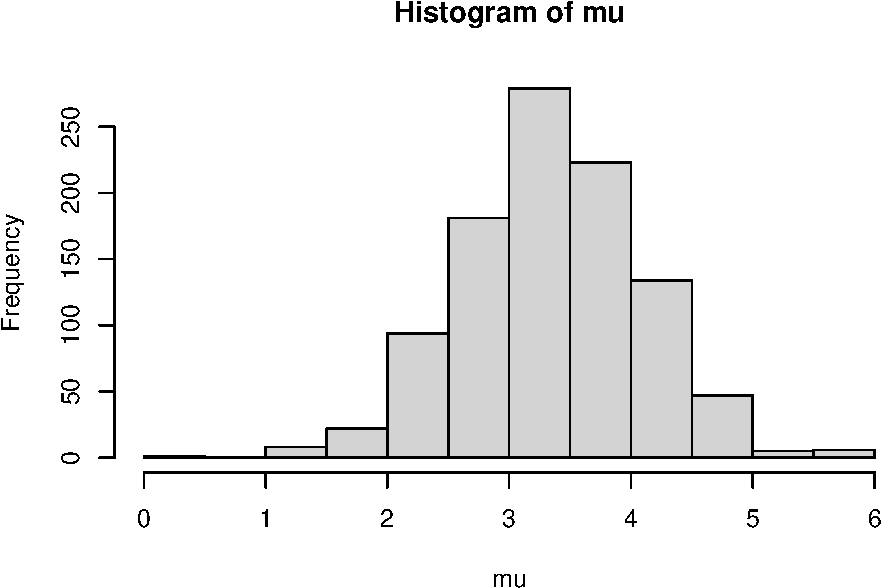
\includegraphics[width=0.5\linewidth]{tutorial_files/figure-latex/unnamed-chunk-10-1}

\begin{Shaded}
\begin{Highlighting}[]
\FunctionTok{hist}\NormalTok{(sigma)}
\end{Highlighting}
\end{Shaded}

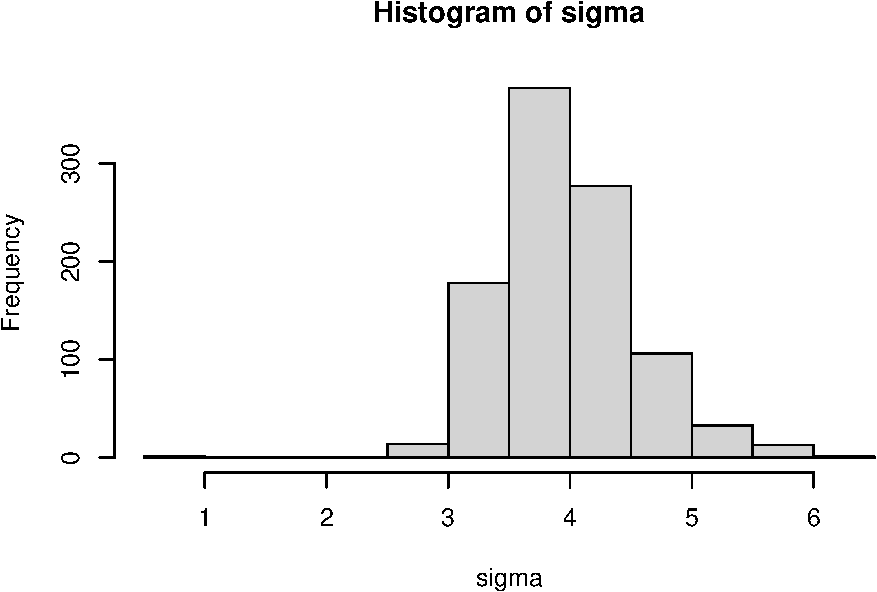
\includegraphics[width=0.5\linewidth]{tutorial_files/figure-latex/unnamed-chunk-10-2}

\begin{Shaded}
\begin{Highlighting}[]
\CommentTok{\# Traceplots}
\FunctionTok{plot}\NormalTok{(mu,}\AttributeTok{t=}\StringTok{"l"}\NormalTok{,}\AttributeTok{bty=}\StringTok{"l"}\NormalTok{)}
\end{Highlighting}
\end{Shaded}

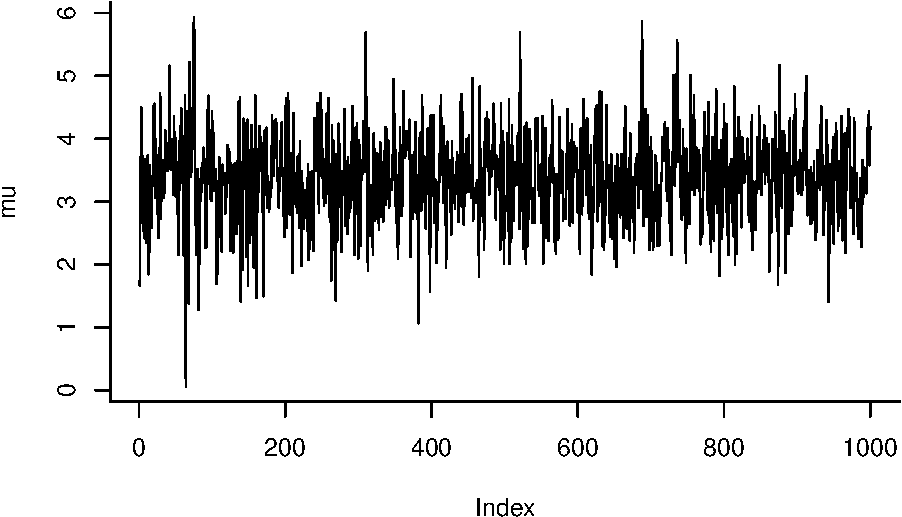
\includegraphics[width=0.5\linewidth]{tutorial_files/figure-latex/unnamed-chunk-11-1}

\begin{Shaded}
\begin{Highlighting}[]
\FunctionTok{plot}\NormalTok{(sigma,}\AttributeTok{t=}\StringTok{"l"}\NormalTok{,}\AttributeTok{bty=}\StringTok{"l"}\NormalTok{)}
\end{Highlighting}
\end{Shaded}

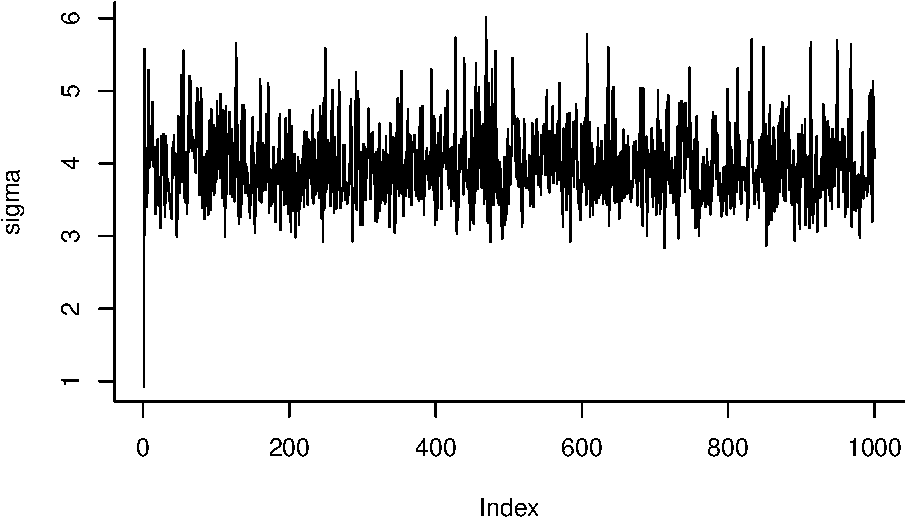
\includegraphics[width=0.5\linewidth]{tutorial_files/figure-latex/unnamed-chunk-11-2}

Once again, notice how powerful MCMC is: technically, you may not model
directly a (highly non-linear) function of the main parameters; for
example, all the computation is made in terms of the precision
\texttt{tau}, although you may be much more interested in learning the
standard deviation sigma. MCMC lets you obtain all the relevant informa-
tion on the latter by simply creating simulations from the posterior
distributions using the relevant inverse function
\texttt{sigma\ =\ 1/sqrt(tau)}.

We can also depict the trajectories of the MCMC samples in the first 10
iterations of the proecess. The arrows follow the moves of the Markov
chain during the updates of the parameters, from the initial

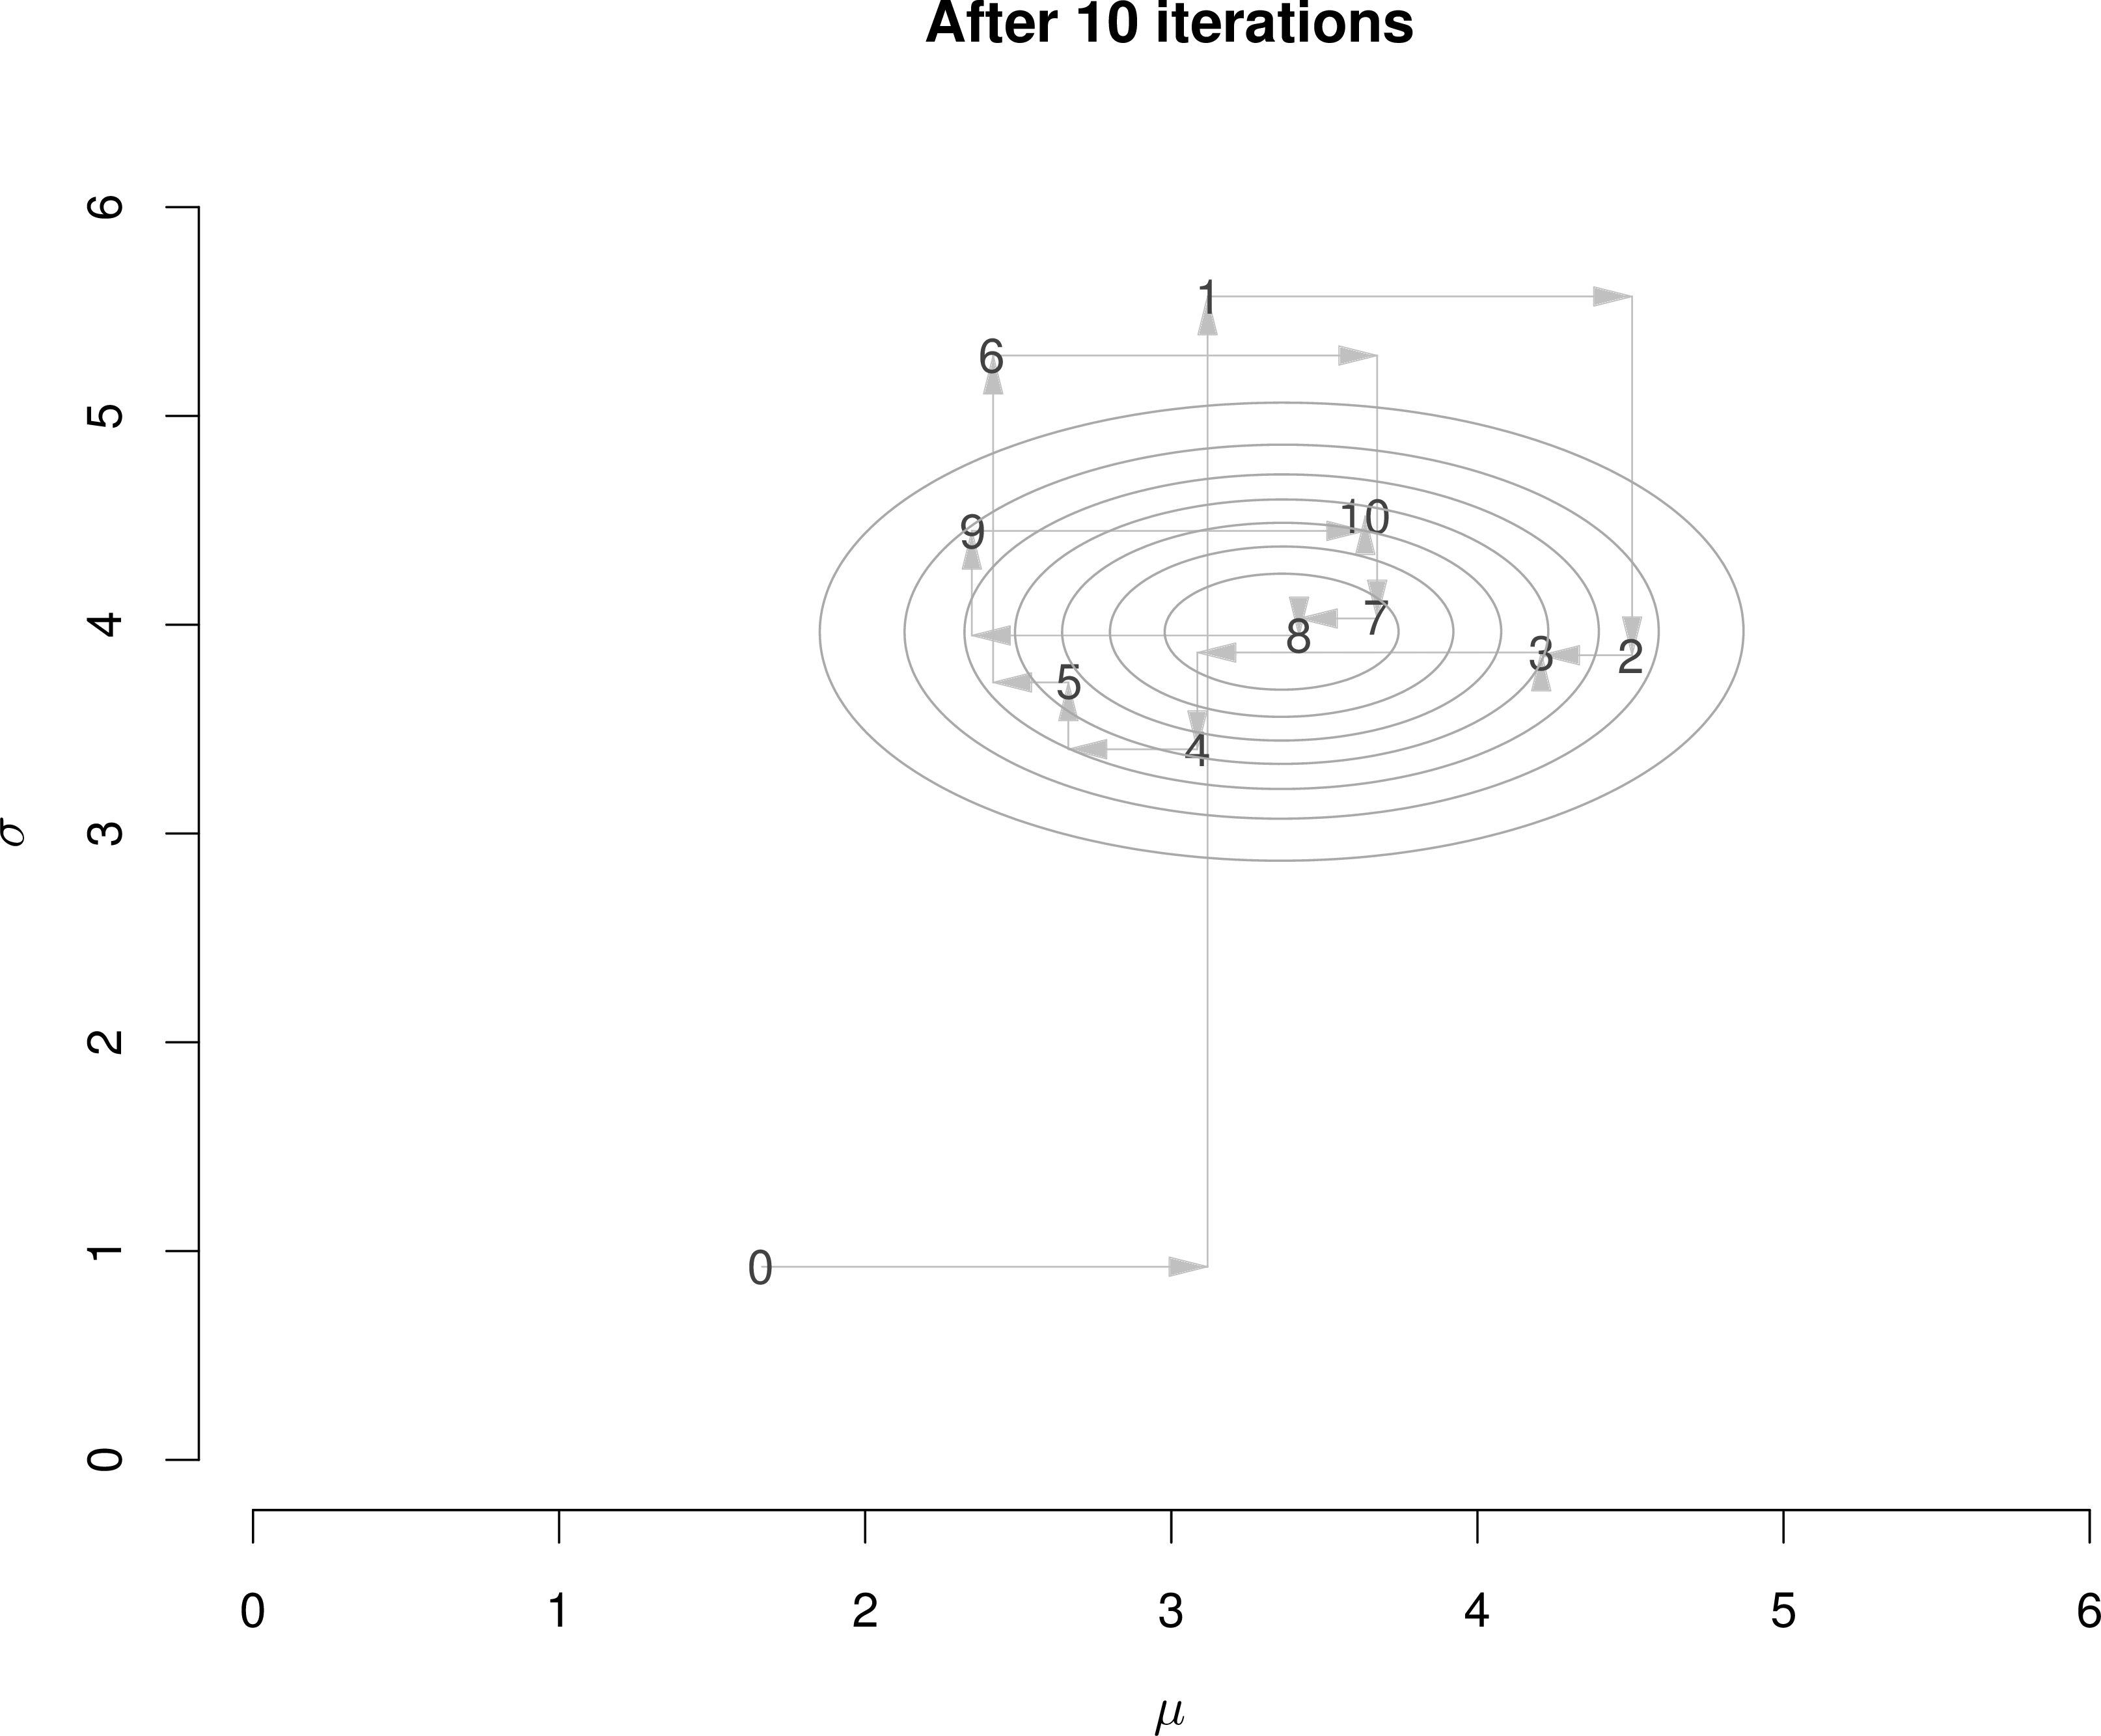
\includegraphics[width=0.5\textwidth,height=\textheight]{/practical/02_mcmc/tutorial_files/figure-html/unnamed-chunk-19-1.png}

\end{document}
